\documentclass{beamer}
%\documentclass[handout]{beamer}
% This file is a solution template for:

% - Giving a talk on some subject.
% - The talk is between 15min and 45min long.
% - Style is ornate.

% Copyright 2004 by Till Tantau <tantau@users.sourceforge.net>.
%
% In principle, this file can be redistributed and/or modified under
% the terms of the GNU Public License, version 2.
%
% However, this file is supposed to be a template to be modified
% for your own needs. For this reason, if you use this file as a
% template and not specifically distribute it as part of a another
% package/program, I grant the extra permission to freely copy and
% modify this file as you see fit and even to delete this copyright
% notice. 


\mode<presentation>
{
  \usetheme{Montpellier}

  %\setbeamercovered{transparent}
  % or whatever (possibly just delete it)
}

\usepackage{xmpmulti} % package that defines \multiinclude

\usepackage[english]{babel}

\usepackage[latin1]{inputenc}

\usepackage{times}
\usepackage[T1]{fontenc}
% Or whatever. Note that the encoding and the font should match. If T1
% does not look nice, try deleting the line with the fontenc.

\title[\ouralg] % (optional, use only with long paper titles)
{Online learning using Bregman Divergences}

\author[Freund] % (optional, use only with lots of authors)
{Yoav Freund}
% - Give the names in the same order as the appear in the paper.
% - Use the \inst{?} command only if the authors have different
%   affiliation.

\institute[Universities of Somewhere and Elsewhere] % (optional, but mostly needed)

\subject{Machine Learning}
% This is only inserted into the PDF information catalog. Can be left
% out. 

% If you have a file called "university-logo-filename.xxx", where xxx
% is a graphic format that can be processed by latex or pdflatex,
% resp., then you can add a logo as follows:

% \pgfdeclareimage[height=0.5cm]{university-logo}{university-logo-filename}
% \logo{\pgfuseimage{university-logo}}



% Delete this, if you do not want the table of contents to pop up at
% the beginning of each subsection:
%% \AtBeginSubsection[]
%% {
%%   \begin{frame}<beamer>
%%     \frametitle{Outline}
%%     \tableofcontents[currentsection,currentsubsection]
%%   \end{frame}
%% }


% If you wish to uncover everything in a step-wise fashion, uncomment
% the following command: 

\beamerdefaultoverlayspecification{<+->}

% \newcommand{\R}[1]{{\color{red}{#1}}}
% \newcommand{\W}{\vec{W}}
% \newcommand{\V}{\vec{V}}
% \newcommand{\X}{\vec{X}}
% \newcommand{\loss}{\vec{\ell}}
% \newcommand{\HedgeLoss}{L_{\mbox{\footnotesize Hedge}}}

\newcommand{\newmcommand}[2]{\newcommand{#1}{{\ifmmode {#2}\else\mbox{${#2}$}\fi}}}
\newcommand{\renewmcommand}[2]{\renewcommand{#1}{{\ifmmode {#2}\else\mbox{${#2}$}\fi}}}
\newcommand{\newmcommandi}[2]{\newcommand{#1}[1]{{\ifmmode {#2}\else\mbox{${#2}$}\fi}}}
\newcommand{\newmcommandii}[2]{\newcommand{#1}[2]{{\ifmmode {#2}\else\mbox{${#2}$}\fi}}}
\newcommand{\newmcommandiii}[2]{\newcommand{#1}[3]{{\ifmmode {#2}\else\mbox{${#2}$}\fi}}}

\newcommand{\algfnt}{\bf}

\newmcommand{\ouralg}{{\mbox{\algfnt Hedge}({\eta})}}

\newmcommand{\iter}{T}

\newfont{\cmmib}{cmmib10}
\newcommand{\boldell}{{\mbox{\cmmib \symbol{'140}}}}


\newmcommandi{\costvec}{{\boldell}_{#1}}
\newmcommandii{\cost}{{\ell}^{#1}_{#2}}

\newmcommandi{\rd}{\tilde{#1}}

\newmcommandi{\distvec}{{\bf p}^{#1}}
\newmcommandi{\rddistvec}{\rd{\bf p}^{#1}}
\newmcommandii{\dist}{{p}^{#1}_{#2}}
\newmcommandii{\rddist}{\rd{p}^{#1}_{#2}}

\newmcommandi{\bdistvec}{{\bf q}^{#1}}
\newmcommandii{\bdist}{{q}^{#1}_{#2}}

\newmcommandi{\wtvec}{{\bf w}^{#1}}
\newmcommandi{\rdwtvec}{\rd{\bf w}^{#1}}
\newmcommandii{\wt}{{w}^{#1}_{#2}}
\newmcommandii{\rdwt}{\rd{w}^{#1}_{#2}}


\newcommand{\Nweight}[2]{V_{#1}^{#2}}	%the normalized weight
\newcommand{\dweight}[2]{w^{#2}(#1)} % initial density measure
\newcommand{\TEloss}[1]{L_{#1}}	%total loss of expert i
\newcommand{\BEloss}{L_{\min}}	%total loss of the best expert
\newcommand{\TAloss}{L_A}	%total loss of algorithm
\newcommand{\weight}[2]{W_{#1}^{#2}} % weight assigned to expert
\newcommand{\btheta}{\hat{\theta}}

\newcommand{\R}[1]{{\color{red}{#1}}}
\newcommand{\B}[1]{{\color{blue}{#1}}}
\newcommand{\RM}[1]{{\color{red}{$#1$}}}


%BANDITS
\newcommand{\Aplay}{{\bf Hedge}}
\newcommand{\Aest}{{\bf Exp3}}
\newcommand{\Aesthp}{{\bf Exp3.P}}
\newcommand{\Aestg}{{\bf Exp3.P.1}}
\newcommand{\Aests}{{\bf Exp3.S}}
\newcommand{\Aessg}{{\bf Exp3.S.1}}
\newcommand{\Astrat}{{\bf Exp4}}
\newcommand{\Abound}{{\bf Exp3.1}}
\newcommand{\Gbest}{G_{\rm max}}

\newcommand{\defeq}{\stackrel{\rm def}{=}}
\newcommand{\compl}{\mbox{\sc h}}
\newcommand{\theset}[2]{\{ {#1} \,:\, {#2} \}}

\newmcommandii{\stratv}{\mbox{\boldmath $\xi$}^{#1}({#2})}

%Games paper
\newmcommand{\M}{\bf M}
\newmcommand{\dM}{\M'}
\newmcommand{\Row}{\bf R}
\newmcommand{\dRow}{\R'}
\newmcommand{\C}{\bf C}
\newmcommand{\dC}{\C'}
\newmcommand{\D}{D}
\renewmcommand{\P}{\bf P}
\newmcommand{\Q}{\bf Q}
\newmcommand{\Dt}{\D_t}
\newmcommand{\Pt}{\P_t}
\newmcommand{\Qt}{\Q_t}
\newmcommand{\Pstar}{\P^*}	% the min/max optimal mixed strategy
\newmcommand{\Pref}{\tilde{\P}}	% a reference mixed strategy (not
				% necessarily min/max)
\newmcommand{\Qstar}{\Q^*}
\newmcommand{\Pa}{\overline{\P}}
\newmcommand{\Qa}{\overline{\Q}}
\newmcommand{\Qh}{\hat{\Q}}
\newmcommandi{\trans}{{#1}^{\rm T}}
\newmcommand{\mhx}{\M(h,x)}
\newmcommand{\mxh}{\dM(x,h)}
\newmcommand{\mpq}{\M(\P,\Q)}
\newmcommand{\mpsq}{\M(\Pstar,\Q)}
\newmcommand{\mpsqt}{\M(\Pstar,\Qt)}
\newmcommand{\mptqt}{\M(\Pt,\Qt)}
\newmcommand{\mptt}{\M(\Pt,t)}
\newmcommand{\mptq}{\M(\Pt,\Q)}
\newmcommand{\mpqt}{\M(\P,\Qt)}
\newcommand{\minp}{\min_{\P}}
\newcommand{\maxq}{\max_{\Q}}
\newcommand{\RE}[2]{{\rm RE}\left( {#1} \; \parallel \; {#2} \right) }

\newmcommand{\sumt}{\sum_{t=1}^T}
\newmcommand{\sumin}{\sum_{i=1}^n}
\newmcommand{\delt}{\Delta_{T,n}}
\newcommand{\nextline}{\vspace{0.2cm}\\}   % a little space for equation arrays

\newcommand{\lwalg}{\mbox{\rm MW}}
\newcommand{\lwalgvar}{\mbox{\rm vMW}}

%%
\newcommand{\E}{\mbox{\rm\bf E}}
\newcommand{\p}[2]{p_{#1}(#2)}
\newcommand{\q}[2]{q_{#1}(#2)}
\newcommand{\x}[2]{x_{#1}({#2})}
\newmcommand{\bx}{\mbox{\boldmath$x$}}
\newmcommandi{\xv}{\bx({#1})}
\newmcommand{\xvt}{\xv{t}}
%\newcommand{\w}[2]{w_{#1}({#2})} replaced by \wt, but remember to switch order of parameters i and t
\renewcommand{\i}[1]{i_{#1}}
\newcommand{\hx}[2]{\hat{x}_{#1}(#2)}
\newcommand{\hxit}{\hx{\i{t}}{t}}
\newcommand{\pit}{\p{\i{t}}{t}}
\newcommand{\xit}{\x{\i{t}}{t}}
\newcommand{\expb}[1]{\exp\left(#1\right)}

\newcommand{\vp}{{\mathbf p}}
\newcommand{\vu}{{\mathbf u}}
\newcommand{\vv}{{\mathbf v}}
\newcommand{\vx}{{\mathbf x}}
\newcommand{\vy}{{\mathbf y}}
\newcommand{\vw}{{\mathbf w}}
\newcommand{\vq}{{\mathbf q}}

\newcommand{\vecq}{{\bf q}}
\newcommand{\vecp}{{\bf p}}


\newcommand{\HedgeLoss}{L_{\mbox{\footnotesize Hedge}}}

\newcommand{\W}{\vec{W}}
\newcommand{\V}{\vec{V}}
\newcommand{\X}{\vec{X}}
\newcommand{\vb}{\vec{b}}
%\newcommand{\loss}{\vec{\ell}}
\newcommand{\loss}{L}
\newcommand{\elloss}[2]{\ell_{#2}\left( #1 \right)} %loss of expert i at time t
\newcommand{\lossvec}[1]{{\mathbf \ell}_{#1}}       %loss of expert at time t
\newcommand{\w}[1]{\makebox[12pt]{{#1}}}
\newcommand{\Rps}{\mbox{\tt R}}
\newcommand{\rPs}{\mbox{\tt P}}
\newcommand{\rpS}{\mbox{\tt S}}
\newcommand{\rpstie}{\w{$\frac{1}{2}$}}
\newcommand{\rpswin}{\w{$0$}}
\newcommand{\rpsloss}{\w{$1$}}

\newmcommand{\decspace}{\Delta}
\newmcommand{\decsym}{\delta}
\newmcommandi{\dec}{\decsym^{#1}}
\newmcommand{\decdistsym}{\cal D}
\newmcommandi{\decdist}{{\decdistsym}^{#1}}

\newmcommand{\simpdistspace}{{\bf \cal S}}
\newmcommand{\domset}{{\rm dom}(\decdistsym)}

\newmcommand{\expdistsym}{{\cal E}}
\newmcommandii{\expdist}{{\expdistsym}^{#1}_{#2}}
\newmcommand{\expdecsym}{{\varepsilon}}
\newmcommandii{\expdec}{\expdecsym^{#1}_{#2}}

\newmcommand{\outspace}{\Omega}
\newmcommand{\outsym}{\omega}
\newmcommandi{\out}{\outsym^{#1}}

%\newmcommandii{\Dkl}{D_{\mbox{kl}}\paren{#1||#2}}
\newmcommandii{\Dkl}{{\rm {KL}}\paren{{#1}\;||\;{#2}}}

\newmcommandi{\sumwts}{\sum_{i=1}^N \wt{#1}{i}}

\newmcommand{\lossalg}{L_A}
\newmcommand{\lossouralg}{{L_{\mbox{\scriptsize\algfnt Hedge}(\eta)}}}
\newmcommand{\lossS}{{L_{\mbox{\scriptsize\algfnt S}}}}
\newmcommandi{\lossi}{L_{#1}}
\newmcommandii{\lossit}{L_{#1}^{#2}}

\newmcommandi{\upbnd}{\tilde{#1}}

\newcommand{\angles}[1]{{\left\langle {#1} \right\rangle}}
\newcommand{\paren}[1]{{\left( {#1} \right)}}
\newcommand{\brac}[1]{{\left[ {#1} \right]}}
\newcommand{\braces}[1]{{\left\{ {#1} \right\}}}

\newcommand{\abs}[1]{{\left| {#1} \right|}}
\newcommand{\ceiling}[1]{{\left\lceil {#1} \right\rceil}}

\newfont{\msym}{msbm10}
\newcommand{\real}{\mbox{\msym R}}

\newmcommand{\updatefcn}{U_\eta}

%% \newtheorem{theorem}{Theorem}	
%% \newtheorem{lemma}[theorem]{Lemma}
%% \newtheorem{corollary}[theorem]{Corollary}
%% \newtheorem{definition}{Definition}

%\newcommand{\proof}{\noindent{\bf Proof:} }
%\newcommand{\example}[1]{{\em Example #1.} }
%\newcommand{\qed}{\rule{0.7em}{0.7em}}

\newcommand{\WeakAlg}{\mbox{\algfnt WeakLearn}}
\newcommand{\Boost}{\mbox{\algfnt AdaBoost}}
\newcommand{\EX}{\mbox{\bf EX}}
\newmcommand{\hf}{h_{{f}}}
\newmcommand{\rdhf}{\rd{h}_{{f}}}
\newmcommand{\hfT}{h^T_{{f}}}
\newmcommand{\ranh}{{b}}

\newmcommand{\conclass}{{\cal C}}

\newmcommand{\badvec}{{\bf b}}
\newmcommandi{\bad}{{b}_{#1}}

%%%%%%%% New commands defined for the game-playing paper

\newmcommand{\hedge}{\algfnt Hedge}
\newmcommand{\play}{\algfnt Play}
\newmcommandi{\Glossvec}{{\bg y}^{#1}}
\newmcommandii{\Gloss}{{y}^{#1}_{#2}}
%\newmcommandi{\action}{{I}_{#1}}
\newmcommandi{\Gdistvec}{{\bf \tilde{p}}^{#1}}
\newmcommandii{\Gdist}{{\teilde{p}}^{#1}_{#2}}

%%%%%%%%%%%%%%%%%%%%%%%%%%%%%%%%%%%%%%%%%%%%%%%%%%%%%
\newmcommand{\Idistvec}{{D}}
\newmcommandi{\Idist}{\Idistvec({#1})}
\newmcommand{\Idistt}{\Idistvec_t}

\newmcommand{\Xdist}{{\cal P}}
\newmcommand{\emp}{\hat{\epsilon}}

\newmcommand{\classpc}{Y}
\newmcommand{\numclass}{k}
\newmcommandii{\prob}{\mbox{\rm Pr}_{#1}\left[{#2}\right]}
\newmcommandii{\exval}{\mbox{\rm E}_{#1}\left[{#2}\right]}

%\usepackage{amsmath}
\DeclareMathOperator*{\argmax}{argmax} % thin space, limits underneath in displays
\DeclareMathOperator*{\argmin}{argmin} 

\newcommand{\RR}{\mathbb{R}}
\newcommand{\regret}{\mbox{Regret}}

%%% Conditional probabilities
\newmcommandii{\condp}{p\left( #1 \left| #2 \right. \right)}

\newmcommand{\lab}{y}
\newmcommand{\ploss}{\mbox{ploss}}
\newmcommandii{\avploss}{\ploss_{#1}({#2})}
\newcommand{\sfrac}[2]{\mbox{$\frac{#1}{#2}$}}

\newcommand{\mboosta}{\mbox{\algfnt AdaBoost.M1}}
\newcommand{\mboostb}{\mbox{\algfnt AdaBoost.M2}}
\newcommand{\mboostr}{\mbox{\algfnt AdaBoost.R}}

%\newmcommand{\slos}{\mbox{ploss}}
%\newmcommandiii{\sloss}{\slos_{#1}({#2},{#3})}
%\newmcommandiii{\avsloss}{\slos_{{#1},{#2}}({#3})}

\newmcommandii{\vwt}{{W}^{#1}_{#2}}

\newcommand{\figline}{\rule{\textwidth}{1pt}}

%\newmcommandi{\1}{{\bf 1}({#1})}
\newmcommandi{\1}{[\![{#1}]\!]}

\newmcommand{\confcn}{\kappa}
\newmcommandi{\erint}{\abs{\int_{y_i}^{h_t(x_i)} {#1} dy}}
%\newmcommandi{\erint}{\int_{\min\{y_i,h_t(x_i)\}}^{\max\{y_i,h_t(x_i)\}}{#1}dy}


\begin{document}

%\iffalse %%%%%%%%%%%%%%%%%%%%%%%%%%%%%%%%%%%%%%%%%%%%%%%%%%%%%%%%%%%%%%%%%%
%\fi %%%%%%%%%%%%%%%%%%%%%%%%%%%%%%%%%%%%%%%%%%%%%%%%%%%%%%%%%%%%%%%%%%%

\begin{frame}
  \titlepage
  \begin{small}
    Material follows Chapter 11 of ``Prediction Learning and
    Games'' and ``Adaptive game playing using multiplicative weights''
    by Freund and Schapire.
  \end{small}
\end{frame}

\begin{frame}
  \frametitle{Outline}
  \tableofcontents[pausesections]
  % You might wish to add the option [pausesections]
\end{frame}


\section{\ouralg Algorithm}

\begin{frame}
\frametitle{The hedging problem}

\begin{itemize}
\item \R{$N$} possible actions 

\item At each time step \R{$t=1,2,\ldots,T$}:
\begin{itemize}
\item Algorithm chooses a distribution \R{$\distvec{t}$} over actions.
\item Losses \R{$0 \leq \cost{t}{i} \leq 1$} of all actions \R{$i=1,\ldots,N$} are revealed.
\item Algorithm suffers {\bf expected} loss \R{$\distvec{t} \cdot \costvec{t}$}
\end{itemize}
\item {{\bf Goal:} minimize total expected loss}
\item {Here we have stochasticity - but only in {\bf algorithm}, not in {\bf outcome}}
\end{itemize}
\end{frame}

\begin{frame}
\frametitle{The \ouralg Algorithm}
~\\
Consider action \R{$i$} at time \R{$t$}
\begin{itemize}
\item Total loss:
\R{$$L_i^t = \sum_{s=1}^{t-1} \ell_i^s$$}
\item Weight:
\R{$$\wt{t}{i} = \wt{1}{i} e^{-\eta L_i^t}$$}
Note freedom to choose initial weight (\R{$\wt{1}{i}$})
\R{$\sum_{i=1}^n \wt{1}{i} = 1$}.
\item
\R{$\eta>0$} is the learning rate parameter. Halving: \R{$\eta \to \infty$}

\item Probability:
\R{$$\dist{t}{i} = \frac{\wt{t}{i}}{\sum_{j=1}^N \wt{t}{i}},\;\;
  \pause     \distvec{t} = \frac{\wtvec{t}}{\sum_{j=1}^N \wt{t}{i}}$$}
\end{itemize}
\end{frame}

\section{Bound on total loss}
\begin{frame}
\frametitle{Bound on the loss of \ouralg Algorithm}
\begin{itemize}
\item
\begin{theorem}[main theorem] \label{thm:basic-bnd}
For any sequence of loss vectors \R{$\costvec{1},\ldots,\costvec{\iter}$},
and for any \R{$i\in\{1,\ldots,N\}$}, we have
\R{\begin{equation*}
\lossouralg \leq \frac{-\ln(\wt{1}{i}) + \eta \lossi{i}}
		      {1-e^{-\eta}}.
\end{equation*}}
%% More generally, for any nonempty set $S\subseteq\{1,\ldots,N\}$, we have
%% \begin{equation}\label{eqn:set-bnd}
%% \lossouralg \leq \frac{-\ln(\sum_{i\in S}\wt{1}{i})
%% 			 - \eta \max_{i\in S} \lossi{i}}
%% 		      {1-e^{-eta}}.
%% \end{equation}
\end{theorem}
\item
\R{Proof}: by combining upper and lower bounds on \R{$\sumwts{\iter+1}$}
\end{itemize}
\end{frame}


\begin{frame}
  \frametitle{Comparing with the best distribution}
  \begin{itemize}
  \item {\bf Comparison class:} single experts.
    hindsite.
  \item Does not take advantage of multiple good experts.
  \item We will get tighter bounds by increasing the comparison class
    to include all {\bf convex combinations} of the experts.
  \end{itemize}
\end{frame}

\begin{frame}
\frametitle{Recall Single step bound for \ouralg}
The total weight has to decrease if the loss is large
\R{\[
\sumwts{t+1} \leq  \paren{\sumwts{t}} \left( 1-(1-e^{-\eta}) \distvec{t}\cdot\costvec{t} \right)
\]}
\end{frame}

\begin{frame}
  \frametitle{Enlarging the comparison set}
  \begin{itemize}
  \item Bound compares cumulative loss to that of best expert in
    hindsite.
  \item Does not take advantage of multiple good experts.
  \item We will get tighter bounds by comparing to the best convex
    combination of experts.
  \end{itemize}
\end{frame}



\begin{frame}
  \frametitle{Comparing with the best distribution}
  \begin{itemize}
  \item Denote by \R{$\vecq$} an arbitrary distribution over \R{$N$}
    experts. \R{$\vecq \in \Delta^N$}. Distribution = convex combination.
  \item Compare loss of algorithm to loss of best
    convex combination of experts:
  \R{\[ \sum_{t=1}^T L_A^t \leq + a \min_{\vecq \in
        \Delta^N} \sum_{t=1}^T \vecq \cdot \costvec{t} + c X \]}
  \item When comparing to single best expert \R{$X=\log N$}
  \item \B{\bf Intuition:} \R{$X$} should be small if best distribution
    \R{$\vecq^*$} is \B{close} to initial distribution \R{$\distvec{0}$}
  \end{itemize}
\end{frame}

\begin{frame}
    \frametitle{Relative Entropy Bound}
    \begin{itemize}
  \item Relative Entropy or KL-Divergence:
    \R{$$\RE{\vecq}{\vecp} \doteq \sum_{i=1}^N \vecq(i) \ln \frac{\vecq(i)}{\vecp(i)}$$}
  \item For any distribution \R{$\vecq$} and any learning rate \R{$\eta>0$} The
    cumulative loss of \B{$\ouralg$} is bounded by:
    \R{\[
      \sum_{t=1}^T \vecp_t \cdot \costvec{t} \leq a_{\eta}\;
      \sum_{t=1}^T \vecq \cdot \costvec{t} +c_{\eta}\;\RE{\vecq}{\vecp_0}
    \]}
  \item Where \R{$a_\eta = \frac{\eta}{1-e^{-\eta}},\;\; c_\eta = \frac{1}{1-e^{-\eta}}$}
  \end{itemize}
\end{frame}

\begin{frame}
\frametitle{Per Iteration bound}
\begin{itemize}
    \item For any distribution \R{$\vecq$} and any iteration \R{$t$}
    \B{$\ouralg$}:
    \R{\[
        c_{\eta}\; \left(\RE{\vecq}{\vecp_{t}} - \RE{\vecq}{\vecp_{t+1}}
        \right) \geq
        \vecp_t \cdot \costvec{t}
        - a_{\eta}\; \vecq \cdot \costvec{t}
      \]}
\end{itemize}
\end{frame}

\begingroup
\small
\begin{frame}
\frametitle{Proof (from RE to ratio)}
\begin{eqnarray*}
\lefteqn{\RE{\vecq}{\vecp_{t}} - \RE{\vecq}{\vecp_{t+1}}} \cr
  &=& \sum_{i=1}^N \vecq(i) \ln \frac{\vecq(i)}{\vecp_t(i)} -
      \sum_{i=1}^N \vecq(i) \ln \frac{\vecq(i)}{\vecp_{t+1}(i)} \cr
  & = & \sum_{i=1}^N \vecq(i) \ln \frac{\vecp_{t+1}(i)}{\vecp_t(i)}
        \cr
  & = & \sum_{i=1}^N \vecq(i) \ln \frac{\exp \left( -\eta
        \costvec{t}(i) \right)}{Z_t}
\end{eqnarray*}
Because
\[
\vecp_{t+1}(i) = \vecp_{t}(i)
\frac{e^{-\eta \costvec{t}(i)}}{Z_t};\;\;\;
Z_t = \sum_{i=1}^N \vecp_t(i)
        \exp( -\eta \costvec{t}(i))
  \]
\end{frame}

\begin{frame}
\frametitle{Proof (from ratio to bound)}
\begin{eqnarray*}
\lefteqn{\sum_{i=1}^N \vecq(i) \ln \frac{\exp \left( -\eta
  \costvec{t}(i) \right)}{Z_t}} \cr
  &=& -\eta \vecq \cdot \costvec{t} - \ln Z_t \cr
  &\geq& -\eta \vecq \cdot \costvec{t} - \ln\left[ \sum_{i=1}^N
         \vecp_t(i) \left(1-(1-e^{-\eta})\costvec{t}(i)
         \right)\right] \cr
  && \mbox{because } e^{-\eta x} \leq (1-(1-e^{-\eta})x) \mbox{ for } x
     \in [0,1] \cr \cr
     & \geq & (1 - e^{-\eta}) \vecp_t \cdot \costvec{t} - \eta \vecq
              \cdot \costvec{q} \cr
  && \mbox{because } \ln (1-x) \leq -x \mbox{ for } x<1
\end{eqnarray*}
\end{frame}

\endgroup

\newcommand{\grad}{\bigtriangledown}

\begin{frame}
\frametitle{Divergence as Potential}
\begin{itemize}
    \item For any distribution \R{$\vecq$} and any iteration \R{$t$}
    \B{$\ouralg$}:
    \R{\[
        \RE{\vecq}{\vecp_{t}} - \RE{\vecq}{\vecp_{t+1}}
        \geq
        \frac{1}{c_\eta} \vecp_t \cdot \costvec{t}
        - \frac{a_{\eta}}{c_\eta}\; \vecq \cdot \costvec{t}
      \]}
\item
  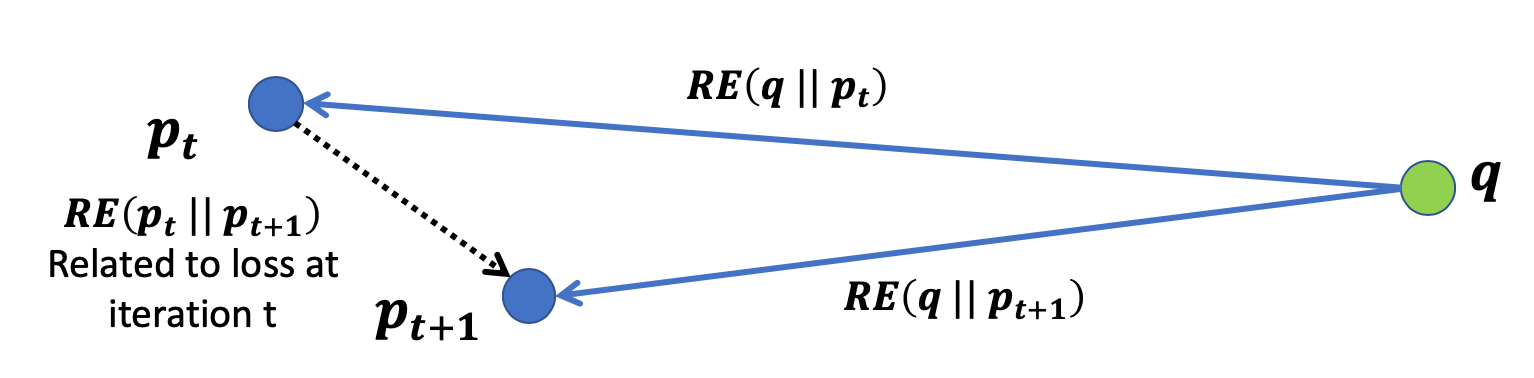
\includegraphics[width=3in]{figures/divergenceAsPotential.png}
\item If the loss of $\vecp_{t}$ is larger than that of $\vecq$ forces
  $\vecp_{t+1}$ do get closer to $\vecq$.
\item The distance from \R{$\vecp_0$} to \R{$\vecq^*$} bounds the total regret. 
\end{itemize}
\end{frame}

\begin{frame}
  \frametitle{online Gradient Descent}
  \begin{itemize}
  \item \R{$\omega_t$} - prediction vector
  \item \R{$x_t$} - outcome vector
  \item \R{$L(\omega,x)$} - loss function (maps prediction,outcome
    to non-negative loss, differentiable)
  \item algorithm suffers \R{$L(\omega_t,x_t)$}
  \item Algorithm updates \R{$\omega_{t+1}= \omega_t - \eta \grad_\omega L_t(x_t\omega_t)$}
  \item Small \R{$\eta$} = small correction = strong regularization.
  \end{itemize}
\end{frame}

\begin{frame}
  \frametitle{Divergence as Regularization}
  \begin{itemize}
  \item Use a divergence term $D(\omega_t,\omega_{t+1})$ to measure
    the size of the update.
  \item Find $\omega_{t+1}$ to balance loss reduction and divergence:
    \R{$$\mbox{argmin}_{\omega} \paren{L(\omega,x_t) + \eta
      D(\omega,\omega_t)}$$}
  \item If update is small, we can think of it in terms of gradients:
    \R{$$\grad_\omega (L(\omega,x_t) + \eta D(\omega,\omega_t))$$}
  \end{itemize}
\end{frame}




\end{document}


